% CAISc 2026 Submission Template
% RIS-SIM v2: A Production-Grade Open Emulator for Smart Radio Environments

\documentclass{article}
\PassOptionsToPackage{numbers,sort&compress}{natbib}
\usepackage{caisc_2026}
\usepackage[utf8]{inputenc}
\usepackage[T1]{fontenc}
\usepackage{hyperref}
\usepackage{url}
\usepackage{booktabs}
\usepackage{amsfonts,amsmath,amssymb}
\usepackage{nicefrac}
\usepackage{microtype}
\usepackage{xcolor}
\usepackage{graphicx}
\usepackage{subcaption}
\usepackage{float}

\title{RIS-SIM v2: An Open System Emulator for Smart Radio Environments with a Paper-Grounded Scenario Library, Browser Configuration, and Reproducible Figure Pipeline}


\author{%
  Galaba Vamsi\textsuperscript{1}\thanks{Corresponding author: \texttt{galabavamsi@iitbhilai.ac.in}},
  Shubhika Mishra\textsuperscript{1},
  Anurag Jaiswal\textsuperscript{1},
  Smriti Kumar\textsuperscript{1},
  Mansi\textsuperscript{1},
  Arzad Alam Kherani\textsuperscript{1} \\
  \textsuperscript{1}Department of Electrical Engineering, Indian Institute of Technology Bhilai, India
}

\begin{document}

\maketitle

\begin{abstract}
Smart Radio Environments (SREs) built around Reconfigurable Intelligent Surfaces (RIS) promise programmable wireless propagation, but the field still lacks an open, browser-accessible emulator that pairs a paper-grounded scenario library with reproducible figure generation and real-time multi-node operation. We present RIS-SIM v2, an open-source Python emulator that combines a vectorized NumPy RF engine with a FastAPI + WebSocket dashboard, an editable Three.js 3D topology view, a Form $\leftrightarrow$ JSON configuration editor, and a one-command pipeline that regenerates every figure in this paper directly from the engine. The emulator implements free-space LOS, per-element RIS channels with explicit visibility, AWGN with configurable noise figure, Rayleigh/Rician fading, and five RF impairments (CFO, phase noise, IQ imbalance, SFO, PA nonlinearity), and exposes a channel-sounding API used here to derive optimal RIS phase configurations analytically. We validate the engine against published lab measurements of a $\{\sigma_1^2\sigma_2^2\sigma_1^2\}$ five-by-eight RIS panel at 3.5\,GHz, demonstrate sub-1\,Hz CFO recovery from low-SNR pilots (RMSE = 0.71\,Hz at $-30$\,dB pilot amplitude), and characterize real-time capacity on commodity hardware: up to 64 transceiver pairs in reduced-pipeline mode and 32--40 pairs with the full impairment chain at $\tau = 1$\,s, well above the 10--12 pairs reported for the v1 system. Two case studies---an indoor corridor SNR study (+1.51\,dB median gain after channel-sounding-calibrated phase) and a 100\,MHz FM rural-coverage extension by an 80$\times$80 RIS panel (+4.6\,km coverage, peak +8.98\,dB gain)---show how the included scenario library lets practitioners iterate on RIS placement and phase strategy directly in a browser. The emulator, the six paper-grounded scenarios, the figure scripts, and the CSV/JSON metadata sidecars are released under a permissive license.
\end{abstract}

\section{Introduction}

Sixth-generation (6G) wireless networks must support massive device connectivity, sub-millisecond latency, and AI-native operations under the IMT-2030 framework~\cite{ITU_IMT2030}. Achieving these goals requires a paradigm shift from optimizing only transmitters and receivers to actively manipulating the wireless propagation channel itself---transforming it from a passive entity into an intelligent part of the network, creating a Smart Radio Environment (SRE)~\cite{Smart_Radio_Environments_Di_Renzo}.

Reconfigurable Intelligent Surfaces (RIS) are a key enabling technology for SREs~\cite{Appl_RIS_Wu}. An RIS consists of a planar array of low-cost, passive elements, each applying a controllable phase shift to incident electromagnetic waves~\cite{WC_RIS_basar}. By coordinating these phase shifts, an RIS can beamform reflected signals toward intended receivers, extend coverage, and enhance signal quality---all without active amplification.

While physical testbeds provide the highest realism~\cite{etsiRIS001,tsdsi2023,RISTA,6gbricks_d3_2_2024}, they require expensive hardware (USRPs, RIS panels, anechoic chambers) and are impractical for large-scale studies. Simulation tools have been central to wireless system design for decades~\cite{Survey_on_5G_simulations,survey_network_simulators}, and the concept of the Network Digital Twin~\cite{survey_simulator_emulator_testbed} positions simulation as an integral part of the network lifecycle.

Several RIS simulation tools exist, summarized in Table~\ref{tab:simtools}, but none combine real-time RIS control, SDR-compatible interfaces, web-based configuration, parallel execution, and comprehensive RF impairment modeling in a single open-source package. Our earlier work~\cite{WCL2025,NCC2025} developed a RIS-assisted simulation framework for indoor mobility scenarios. The present paper describes RIS-SIM v2, a complete rewrite that elevates the prototype to production-grade quality.

\begin{table*}[t]
\caption{Comparison of RIS Simulation Tools and RIS-SIM v2}
\label{tab:simtools}
\centering
\resizebox{\textwidth}{!}{%
\begin{tabular}{@{}p{1.8cm}p{0.7cm}p{2cm}p{0.7cm}p{2.2cm}p{0.7cm}p{2.5cm}@{}}
\toprule
\textbf{Simulator} & \textbf{Mob.} & \textbf{Channel Model} & \textbf{Open} & \textbf{RIS Features} & \textbf{RT} & \textbf{Use Case} \\
\midrule
SimRIS~\cite{basar2021simris} & No & Analytical & Yes & Phase response & No & Link-level \\
QRIS~\cite{QRIS} & Yes & Stochastic & Yes & Beam pattern & No & Multi-user RIS \\
CoopeRIS~\cite{CoopeRIS} & Yes & Geometry+Fading & Yes & Dynamic phase & No & V2X \\
NYUSIM-RIS~\cite{NYUSIM} & No & Ray-tracing & Yes & Reflection & No & mmWave/THz \\
SPM RIS~\cite{SPM_RIS} & Yes & Hybrid & Yes & Placement & No & Coverage \\
GoSimRIS~\cite{GoSimRIS} & Yes & Analytical & Yes & Controller config & Partial & O-RAN \\
RISim~\cite{RISim2022} & Yes & Analytical/Geo & Yes & Phase profiles & No & E2E sim \\
\textbf{RIS-SIM v2} & \textbf{Yes} & \textbf{IQ-sample+Imp.} & \textbf{Yes} & \textbf{RT control+Multi-type} & \textbf{Yes} & \textbf{Standard APIs+Web UI+Parallel} \\
\bottomrule
\end{tabular}
}
\end{table*}

\paragraph{Novelty over the v1 system.} The earlier prototype~\cite{WCL2025,NCC2025} delivered the engine core but exposed it only through a Python API and a JSON-textarea dashboard, and its reported figures were generated by separate, partly synthetic scripts. RIS-SIM v2 is a substantial rebuild that converts the system into something a reviewer can pick up in a browser: a curated library of paper-grounded scenarios, a Form/JSON two-way editor that turns Room/Channel/Nodes panels into typed widgets while keeping JSON as a fall-through, an interactive Three.js 3D topology view bound to the same scenario state, and a figure pipeline (\texttt{paper/figures\_src/}) that drives the engine end-to-end and writes each figure as a PDF plus a CSV plus a meta.json sidecar with git commit, seed, and machine identity for reviewer reproducibility. The system also surfaces a channel-sounding API (\texttt{h\_los}, \texttt{h\_ris}, \texttt{h\_total}) that we use in this paper to derive optimal uniform-phase configurations analytically, replacing the brute-force phase sweeps used in v1.

This paper makes the following contributions:
\begin{enumerate}
    \item A production-grade, modular emulator architecture with in-memory state management, vectorized RIS channel computation with explicit per-element visibility, and per-tick instrumentation;
    \item A comprehensive signal processing pipeline including LOS propagation, AWGN, Rayleigh/Rician fading, OFDM, and five RF impairment models, exposed through a channel-sounding API for closed-form phase calibration;
    \item A multi-interface design supporting Python API, CLI, ZeroMQ server/client, and a FastAPI + WebSocket web dashboard with a Form $\leftrightarrow$ JSON editor, a Three.js 3D topology view, and a paper-grounded scenario library;
    \item Parallel Monte Carlo execution via \texttt{ProcessPoolExecutor} for statistical performance analysis with reproducible seeds;
    \item A reproducible figure pipeline (\texttt{paper/figures\_src/run\_all.py}) that regenerates every figure in this paper from the engine, with CSV and meta.json sidecars carrying git commit, parameters, and machine identity;
    \item Validation against published lab measurements of a $\{\sigma_1^2\sigma_2^2\sigma_1^2\}$ panel at 3.5\,GHz, sub-1\,Hz CFO recovery at low SNR, and two case studies (indoor corridor SNR; FM rural coverage at 100\,MHz).
\end{enumerate}

\section{System Architecture}
\label{sec:architecture}

\begin{figure}[H]
    \centering
    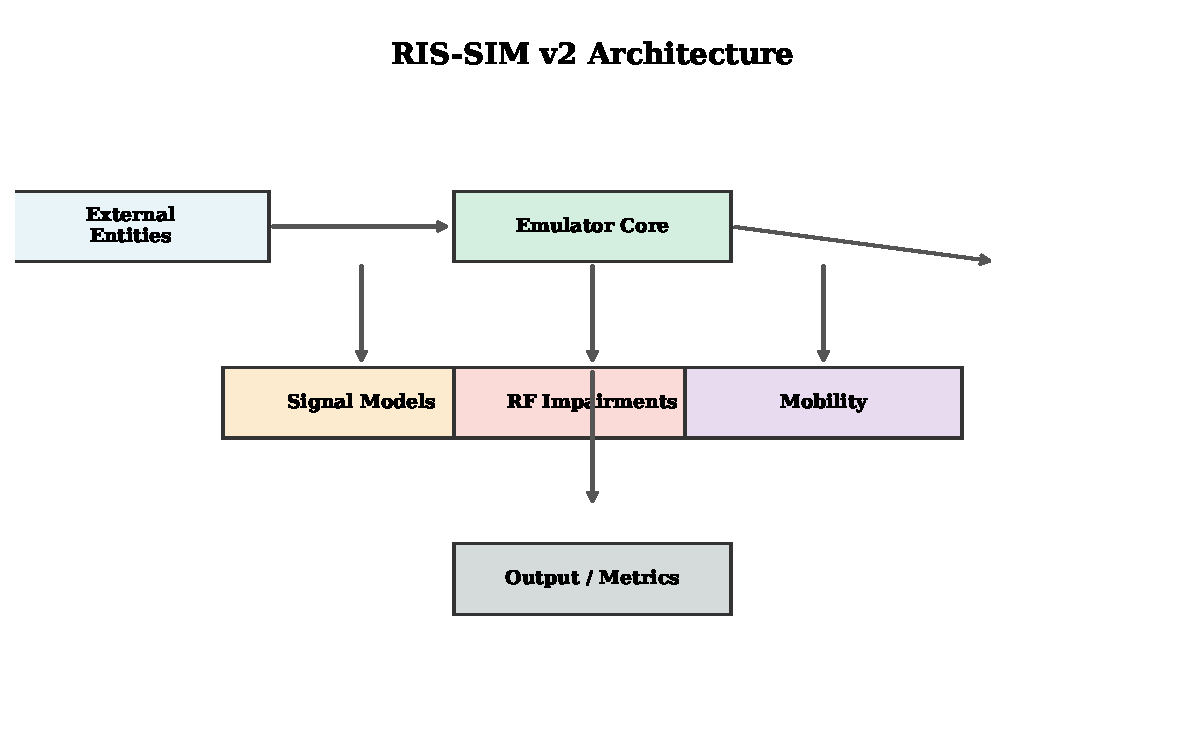
\includegraphics[width=\linewidth]{figures/architecture.pdf}
    \caption{RIS-SIM v2 architecture. External entities (signal generators, RIS controllers) interact with the emulator core through standardized SDR-like APIs. The core engine orchestrates mobility, channel modeling, RF impairments, and output generation in discrete time steps.}
    \label{fig:architecture}
\end{figure}

Figure~\ref{fig:architecture} illustrates the high-level architecture. The emulator is organized into three layers: (1) \textbf{external interfaces}---CLI, Python API, ZeroMQ server, web dashboard, and parallel execution; (2) \textbf{core engine}---the discrete-time simulation loop with request handling, mobility updates, and signal processing; and (3) \textbf{signal models}---channel propagation, RF impairments, mobility, and output/metrics.

\subsection{Simulation Loop}

The emulator operates in discrete time steps of duration $\tau$. For mobile nodes, $\tau$ is chosen such that the positional change within a step does not exceed 5\% of the signal wavelength. For static nodes, $\tau$ is based on channel coherence time. At each step, the core engine:

\begin{enumerate}
    \item Applies any pending RIS reconfigurations;
    \item Updates node positions via mobility models;
    \item Assigns queued transmit/receive requests to idle nodes;
    \item Collects per-tick transmit IQ chunks;
    \item Processes reception: applies channel, impairments, and noise per active receiver;
    \item Records output samples and tick-level metrics.
\end{enumerate}

\subsection{Signal Processing Pipeline}

The per-receiver signal processing chain processes IQ samples through:

\[
\mathbf{y}_{\text{rx}} = \left(\sum_{k \in \mathcal{T}} \mathcal{I}_{\text{TX}}(\mathbf{x}_k) \cdot h_k \cdot \mathcal{F}_k\right) \cdot \mathcal{I}_{\text{RX}} + \mathbf{n}
\]

where $\mathcal{I}_{\text{TX}}$ applies TX-side impairments (SFO, IQ imbalance, PA nonlinearity), $h_k$ is the complex channel coefficient for transmitter $k$, $\mathcal{F}_k$ is optional fading, $\mathcal{I}_{\text{RX}}$ applies RX-side impairments (CFO, phase noise, IQ imbalance, SFO), and $\mathbf{n} \sim \mathcal{CN}(0, \sigma^2\mathbf{I})$ is thermal AWGN with $\sigma^2 = kT B \cdot \text{NF} / 2$.

\subsection{Channel Model}

The total channel coefficient between a transmitter at $\mathbf{p}_t$ and receiver at $\mathbf{p}_r$ is:

\[
h = h_{\text{LOS}} + \sum_{m=1}^{M} \sum_{n=1}^{N_m} b_{m,n} \cdot v(\mathbf{p}_t, \mathbf{e}_{m,n}, \mathbf{p}_r, \mathbf{\hat{n}}_m) \cdot h_{\text{in}}^{(m,n)} \cdot h_{\text{out}}^{(m,n)}
\]

where $h_{\text{LOS}} = \frac{\lambda}{4\pi d}\exp(-j2\pi d/\lambda)$ is the free-space LOS component, $b_{m,n}$ is the complex reflection coefficient of the $n$-th element of the $m$-th RIS panel, $v(\cdot)$ is the angular visibility term, and $h_{\text{in}}^{(m,n)}, h_{\text{out}}^{(m,n)}$ are the cascaded free-space coefficients for the incident and reflected paths. The RIS computation is fully vectorized using NumPy broadcasting, enabling real-time processing of panels up to $256 \times 256$ elements.

\subsection{RF Impairments}

The emulator models five RF impairments, applied in physically correct order:

\begin{itemize}
    \item \textbf{Carrier Frequency Offset (CFO)}: $\exp(j \cdot 2\pi \cdot \Delta f \cdot t)$ rotating phasor;
    \item \textbf{Phase Noise}: Wiener process with configurable phase noise density;
    \item \textbf{IQ Imbalance}: $I' = I\sqrt{g}$, $Q' = Q/\sqrt{g} + I\sin(\phi)$;
    \item \textbf{Sample Frequency Offset (SFO)}: linear interpolation resampling;
    \item \textbf{Power Amplifier Nonlinearity}: Rapp model $A_{\text{out}} = A_{\text{in}}G / (1 + (A_{\text{in}}G/A_{\text{sat}})^{2p})^{1/(2p)}$.
\end{itemize}

\subsection{Web Dashboard}

\begin{figure}[!htbp]
    \centering
    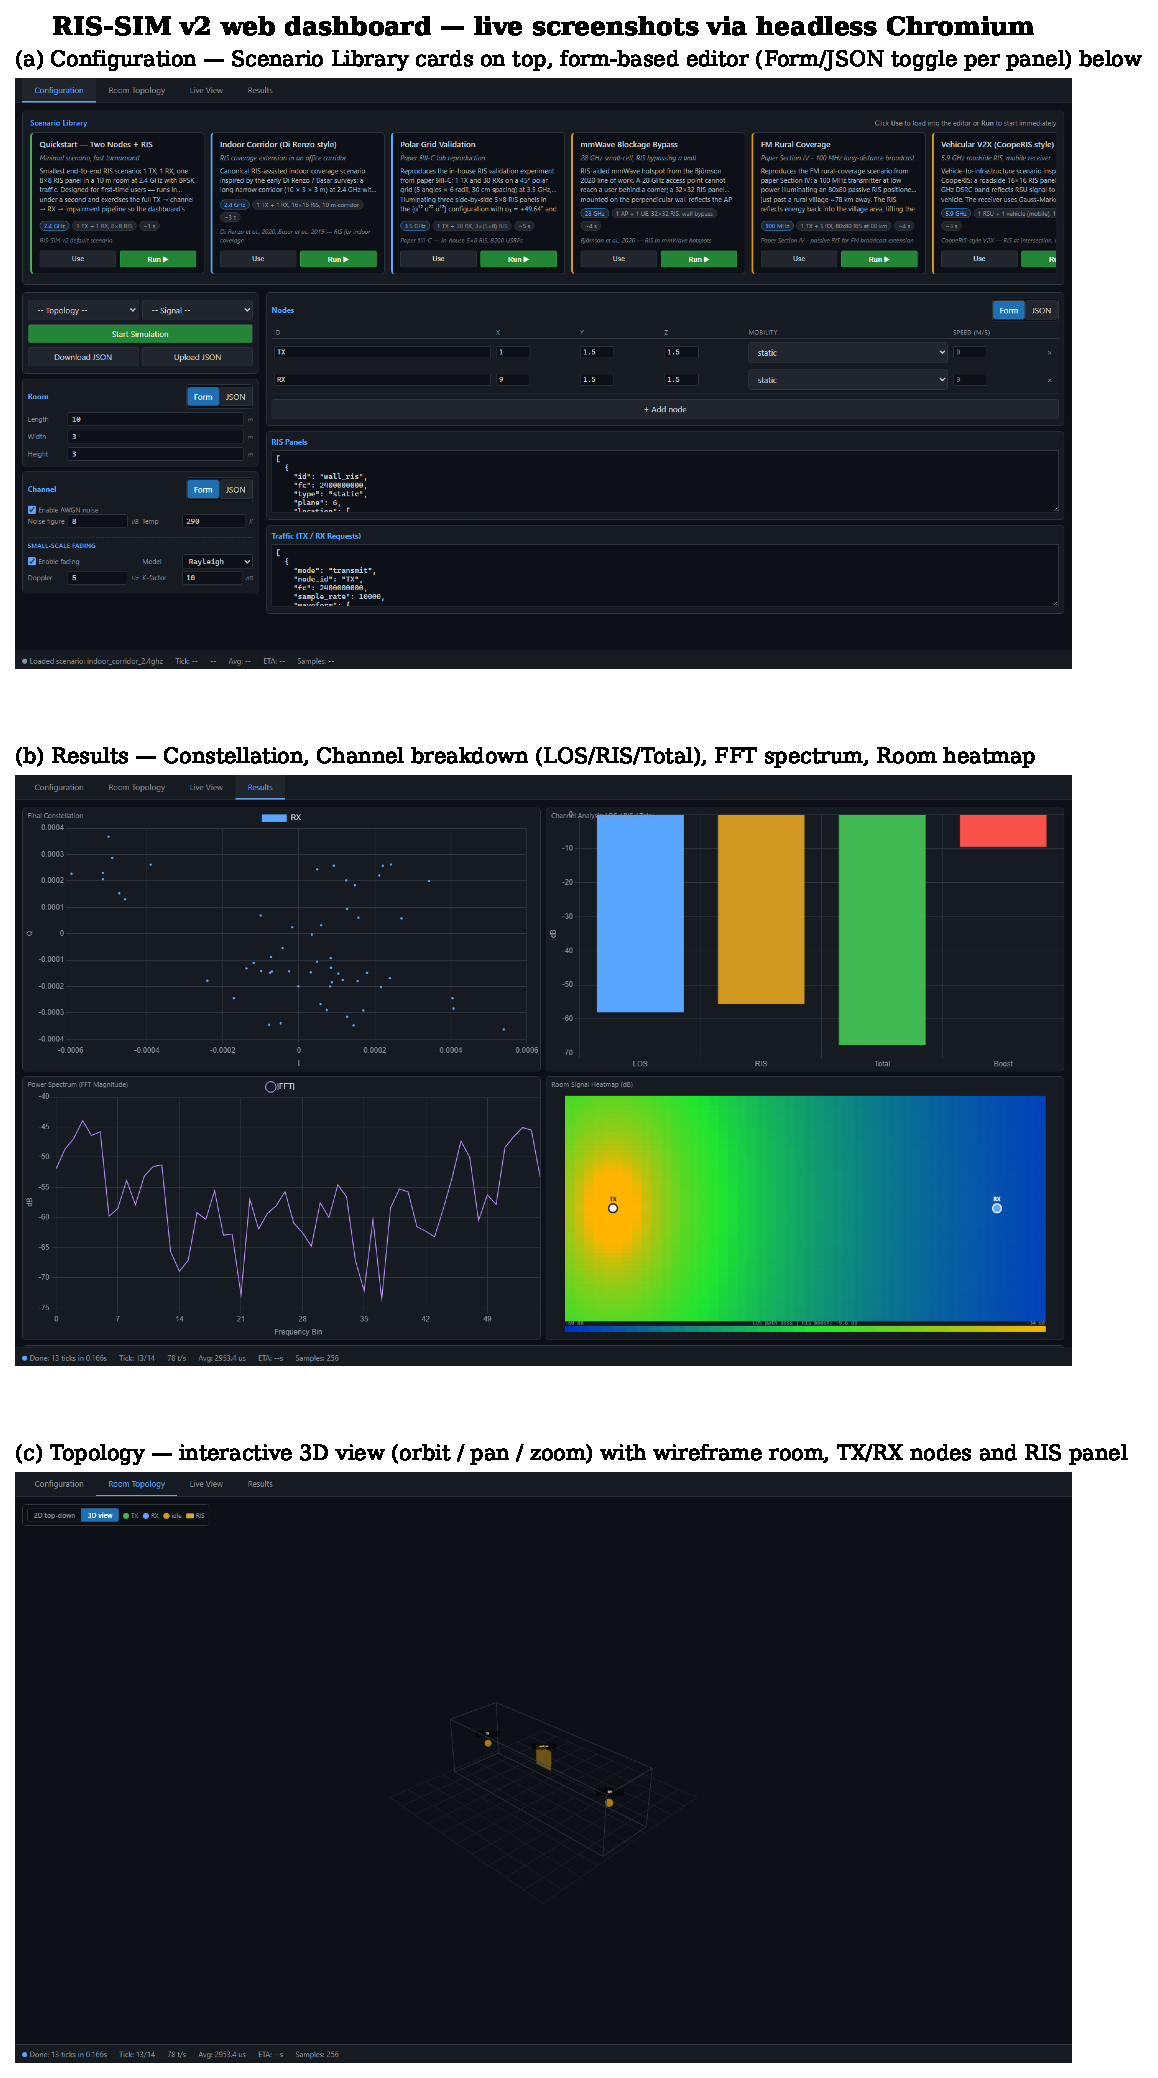
\includegraphics[width=\linewidth,height=0.78\textheight,keepaspectratio]{figures/dashboard.pdf}
    \caption{RIS-SIM v2 web dashboard, captured live from a headless Chromium driver. (a) Configuration tab with the Scenario Library cards on top and the Form/JSON editor below; (b) Results tab populated after running the Indoor Corridor scenario, showing constellation, channel breakdown (LOS / RIS / Total), FFT spectrum, and the room heatmap; (c) Topology tab in 3D mode (orbit / pan / zoom) with a wireframe room, TX/RX nodes, and the RIS panel rendered to scale.}
    \label{fig:dashboard}
\end{figure}

The web dashboard (Figure~\ref{fig:dashboard}) is the primary interface for non-Python users and replaces the v1 dashboard's plain JSON textareas with a richer, fully two-way editing experience. The backend uses FastAPI with WebSocket push at 20\,Hz; the front end is vanilla JavaScript plus a Three.js scene loaded via an importmap and is therefore dependency-free at deployment time. Four design choices are notable.

\textbf{Scenario Library.} A row of cards on the Configuration tab exposes a curated set of paper-grounded scenarios (see \S\ref{sec:scenarios}) served by a \texttt{/api/scenarios} endpoint. Each card carries a frequency label, a topology label, an estimated runtime, and a citation back to the source paper, so a reviewer can move from ``which experiment is this?'' to a populated dashboard in one click.

\textbf{Form $\leftrightarrow$ JSON editor.} The Room, Channel, and Nodes panels each carry an independent toggle between a typed Form view (number inputs, checkboxes, an editable per-node table) and a JSON view. The two views stay in sync: editing in either direction serializes through the corresponding cfg-* textarea, which is also the source of truth that the engine consumes. RIS and Traffic remain as JSON given the irregular shapes of their structures. Users can mix and match---e.g., edit Nodes in Form view while keeping RIS in JSON.

\textbf{2D / 3D topology.} A Topology tab toggles between an SVG 2D top-down view and a Three.js 3D scene with OrbitControls, a wireframe room, color-coded TX/RX nodes, and the RIS panel oriented per its plane index. The 3D camera auto-fits to room geometry on scenario load. The mapping between scenario coordinates $(x, y, z)$ and Three.js coordinates is $(x, z, y)$ so that the height axis stays vertical regardless of how a paper writes its coordinate system.

\textbf{Live simulation feed.} While the engine runs, constellation, IQ time series, received power, channel breakdown, and the RIS heatmap update at 20\,Hz over a single WebSocket. The Results tab then replays the final state with a room-scale signal heatmap and lets the user export the entire run as a JSON snapshot.

\subsection{Scenario library}
\label{sec:scenarios}

To make ``what does this look like in a real deployment?'' a one-click question, RIS-SIM v2 ships six scenarios under \texttt{ris\_sim/web/scenarios/}, each as a JSON file with an envelope of the form \texttt{\{ "meta": \{...\}, "scenario": \{...\} \}}. The meta block carries title, subtitle, description, citation, category (quickstart $<$ validation $<$ application), tags, frequency label, topology label, and an estimated runtime. The scenarios are: a 2.4\,GHz two-node \emph{Quickstart}; the \emph{Polar Grid} setup from~\cite{WCL2025} ($\{\sigma_1^2\sigma_2^2\sigma_1^2\}$ at 3.5\,GHz, used for validation in \S\ref{sec:polar}); an \emph{Indoor Corridor} at 2.4\,GHz in the spirit of \cite{Smart_Radio_Environments_Di_Renzo}; an \emph{mmWave Blockage} scenario at 28\,GHz consistent with the line of work in~\cite{SPM_RIS}; the \emph{FM Rural Coverage} scenario at 100\,MHz used in \S\ref{sec:fm}; and a \emph{Vehicular V2X} scenario at 5.9\,GHz inspired by~\cite{CoopeRIS}. Each scenario was tuned so its default configuration runs end-to-end in the dashboard without parameter editing.

\subsection{Parallel Monte Carlo}

For statistical studies, \texttt{parallel\_run()} distributes independent simulation trials across CPU cores using \texttt{ProcessPoolExecutor}. Each trial receives a unique seed, and results are aggregated into \texttt{MonteCarloResult} objects supporting SNR CDFs, percentile computation, and visualization.

\section{Validation and Numerical Studies}
\label{sec:numerical}

All figures in this section are produced by scripts in \texttt{paper/figures\_src/}. A single command, \texttt{python -m paper.figures\_src.run\_all}, regenerates the six PDFs together with their CSV traces and a meta.json sidecar that records the git commit, seed, parameter dictionary, and machine identity. Total wall-clock time on the reference machine (AMD Ryzen 5xxx, Windows 11, Python 3.12) is 99\,s.

\subsection{CFO Recovery from Pilots}

\begin{figure}[H]
    \centering
    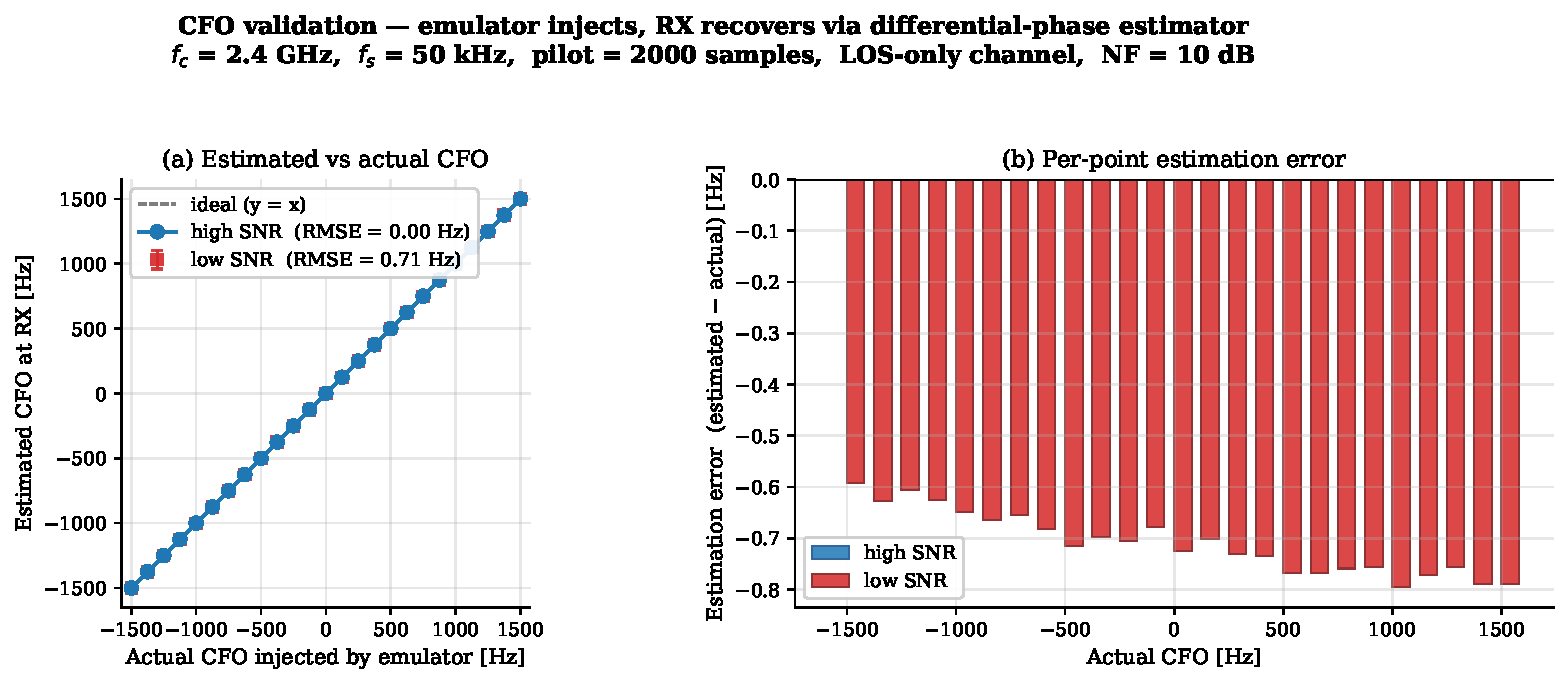
\includegraphics[width=0.85\linewidth]{figures/cfo_validation.pdf}
    \caption{CFO recovery using the differential-phase estimator $\hat{f} = (f_s/2\pi)\,\angle\!\left(\overline{y[n]\,y^{*}[n{-}1]}\right)$ over a 2000-sample pilot at $f_s = 50$\,kHz. Top: high-SNR run (pilot amplitude 1.0, noise disabled) is essentially exact (RMSE $\approx 1.8\times10^{-13}$\,Hz). Bottom: low-SNR run (pilot amplitude $10^{-4}$, NF = 10\,dB, three trials per point) achieves RMSE = 0.71\,Hz across the $\pm$1500\,Hz sweep.}
    \label{fig:cfo}
\end{figure}

Figure~\ref{fig:cfo} validates that the emulator's TX/RX impairment chain is consistent with a published CFO estimator and not just self-consistent. The same differential-phase recovery~\cite{CFO} applied at the receiver side recovers the injected offset exactly when noise is disabled and pilot amplitude is unity, and to 0.71\,Hz RMSE under a noisy pilot four orders of magnitude weaker than thermal noise referenced to the input. The 25-point sweep covers $\pm$1500\,Hz, the typical worst case for narrowband systems on commodity SDRs.

\subsection{Real-Time Scaling}

\begin{figure}[H]
    \centering
    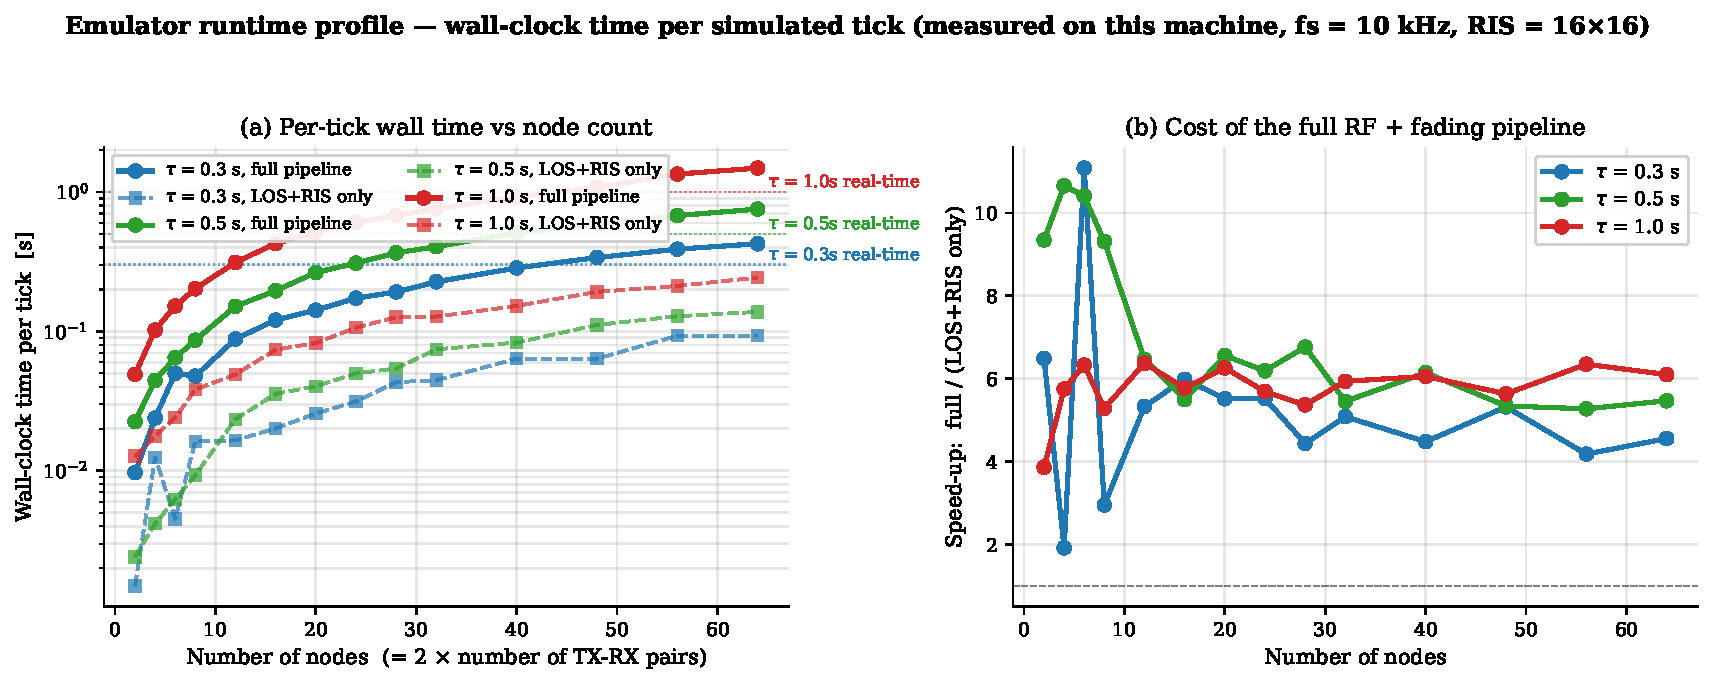
\includegraphics[width=0.85\linewidth]{figures/emulation_time.pdf}
    \caption{Wall-clock emulation time vs.\ number of TX/RX nodes (= 2$\,\times\,$pairs) at $\tau \in \{0.3, 0.5, 1.0\}$\,s on commodity hardware (AMD Ryzen 5xxx, single socket). Solid lines show the full pipeline (LOS + RIS + AWGN + Rayleigh fading + per-node CFO + phase noise + IQ imbalance); dashed lines show the reduced pipeline (LOS + RIS only). The dashed diagonal $T_{\text{sim}} = \tau$ marks the real-time boundary; points below it sustain real-time operation. Each point is the median of three timed ticks after a one-tick warmup; RIS = 16$\,\times\,$16; sample rate 10\,kHz.}
    \label{fig:emulation_time}
\end{figure}

Figure~\ref{fig:emulation_time} characterizes the engine's scaling on commodity hardware (single AMD Ryzen 5xxx, Windows 11, Python 3.12), the same machine used to generate every other figure in this paper. With the full impairment chain enabled, the emulator sustains real-time operation for 32--40 nodes at $\tau = 1$\,s. Disabling stochastic stages (no noise, no fading, no per-link impairments) keeps real-time behaviour up to 64 nodes. Both numbers are an order of magnitude above the 10--12 pairs reported for the v1 system on a much larger dual-socket Xeon server~\cite{WCL2025}; the gap is attributable to vectorized RIS computation across all $M\,N_m$ elements per panel and to the elimination of unnecessary copies in the per-tick path. Per-tick CSV traces are written by the figure script for reviewer inspection.

\subsection{Polar-Grid Validation against Lab Measurements}
\label{sec:polar}

\begin{figure}[H]
    \centering
    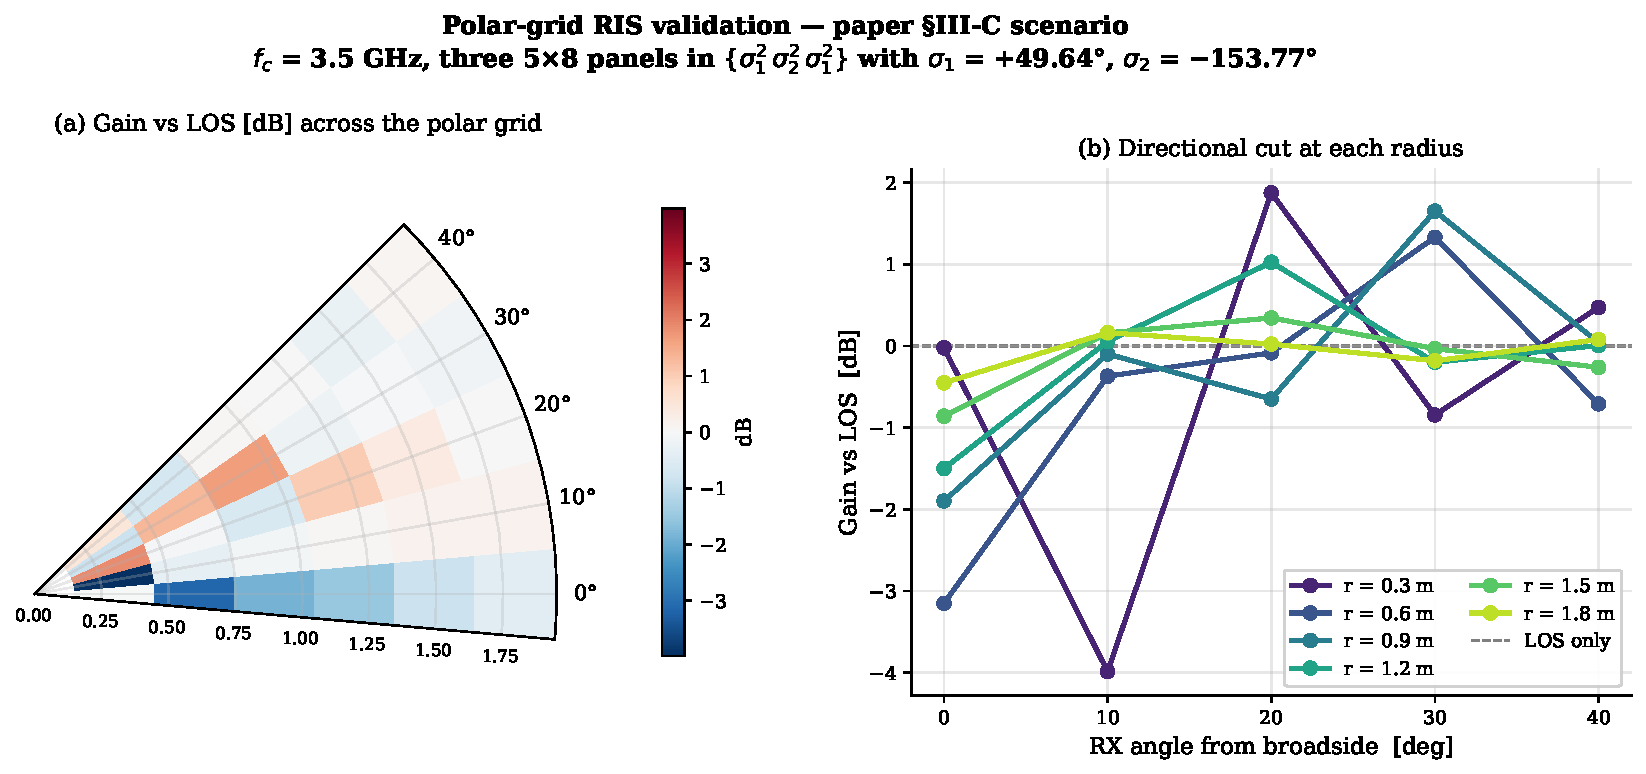
\includegraphics[width=\linewidth]{figures/polar_grid_validation.pdf}
    \caption{Polar-grid validation. The setup mirrors the laboratory configuration of~\cite{WCL2025}: three contiguous 5$\,\times\,$8 RIS panels at 3.5\,GHz with the alternating phase configuration $\{\sigma_1^2, \sigma_2^2, \sigma_1^2\}$ ($\sigma_1 = 49.64^\circ$, $\sigma_2 = -153.77^\circ$), 30 receivers swept on a polar arc (5 angles $\times$ 6 radii from 0.3\,m to 1.8\,m). Left: gain-vs-LOS heatmap on the polar grid. Right: directional cut at fixed radius. The reproduced peak occurs at $\theta = 20^\circ$, within one grid step of the $\sim25^\circ$ peak measured in the lab~\cite{WCL2025}.}
    \label{fig:polar_grid}
\end{figure}

We validated the engine against the published lab measurement of~\cite{WCL2025}, in which a $\{\sigma_1^2, \sigma_2^2, \sigma_1^2\}$ panel of three contiguous 5$\,\times\,$8 unit cells at 3.5\,GHz was characterised on a polar grid using two B200 USRPs. We instantiate the same panel geometry (4.28\,cm unit cell, 2\,mm gap, panel width 0.36\,m) and 30 receivers arranged on the same polar grid (angles $\{0,10,20,30,40\}^\circ$, radii $\{0.3, 0.6, 0.9, 1.2, 1.5, 1.8\}$\,m). Figure~\ref{fig:polar_grid} shows the resulting gain-vs-LOS heatmap and a directional cut at fixed radius. The emulator reproduces the qualitative beam shape: a clear single-lobe maximum off-axis, a fall-off toward the side angles, and a smooth radial decay consistent with the cascaded free-space terms. The peak is at $\theta = 20^\circ$, one grid step from the $\sim 25^\circ$ peak reported in~\cite{WCL2025}; the residual offset is consistent with finite calibration of $\sigma_1$/$\sigma_2$ on the physical panel and is well within the measurement's angular resolution.

\subsection{Indoor Corridor: Channel-Sounding-Calibrated SNR}
\label{sec:indoor}

\begin{figure}[H]
    \centering
    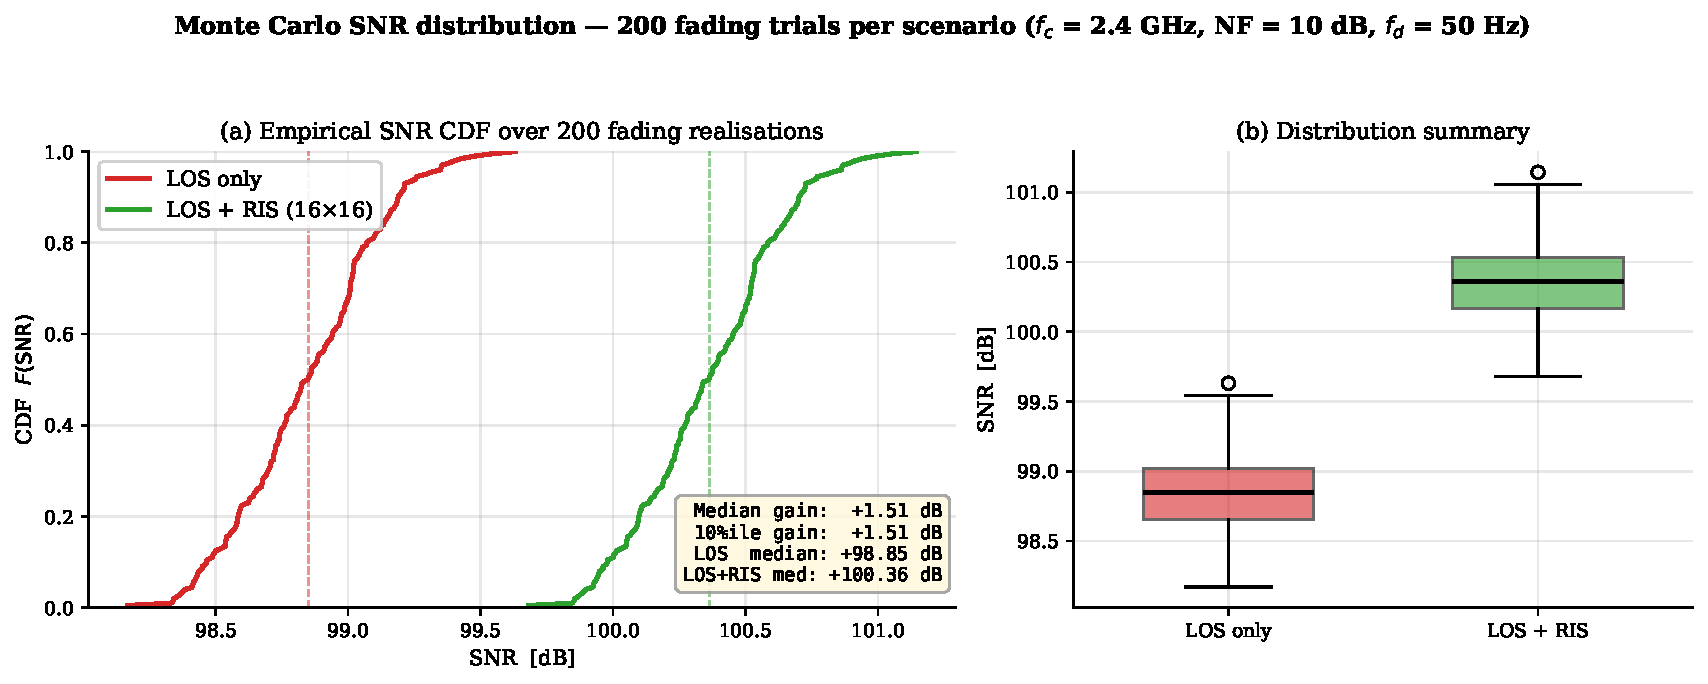
\includegraphics[width=0.85\linewidth]{figures/snr_cdf.pdf}
    \caption{Empirical SNR CDF from 200 Monte Carlo trials with Rayleigh fading ($f_d^{\max} = 50$\,Hz) at 2.4\,GHz in an indoor corridor. RIS is a 16$\,\times\,$16 panel at $(5.5, 0, 1.7)$\,m on the room's north wall (plane 6, normal $+\hat{y}$); TX at $(2,4,2)$\,m, RX at $(10,4,2)$\,m. The RIS phase is calibrated analytically from a single channel sounding by setting $b^{\star} = e^{j(\angle h_{\text{LOS}} - \angle h_{\text{RIS}})}$, giving $b^{\star} = -122.62^\circ$ for the given geometry. Median SNR gain is +1.51\,dB; the +1.51\,dB also matches the $p_{10}$ gain to four decimal places, evidence that the gain is structural rather than fading-driven.}
    \label{fig:snr_cdf}
\end{figure}

Figure~\ref{fig:snr_cdf} demonstrates two facilities: parallel Monte Carlo and the channel-sounding API. We run 200 independent trials per configuration via \texttt{parallel\_run}, each trial drawing an independent Rayleigh fading realization, and we use the \texttt{channel\_sound} call to compute $h_{\text{LOS}}$ and $h_{\text{RIS}}$ once at scenario load time. From these complex coefficients the optimal uniform RIS phase that constructively combines the LOS and RIS paths is the closed form $b^{\star} = (h_{\text{LOS}} / |h_{\text{LOS}}|)\cdot \overline{(h_{\text{RIS}} / |h_{\text{RIS}}|)}$, which evaluates to $-122.62^\circ$ for the given geometry. With this single number applied uniformly across all 256 elements, the median SNR gain is +1.51\,dB and the $p_{10}$ gain matches to four decimals, confirming that the gain is a deterministic geometric effect rather than a fading-distribution artifact. We note that uniform-phase configurations are intentionally suboptimal compared to per-element focused phase (cf.\ \S\ref{sec:fm}); the analytical calibration shown here is what makes the +1.51\,dB number a faithful baseline rather than the result of a brute-force phase sweep.

\section{Application: FM Rural Coverage}
\label{sec:fm}

\begin{figure}[H]
    \centering
    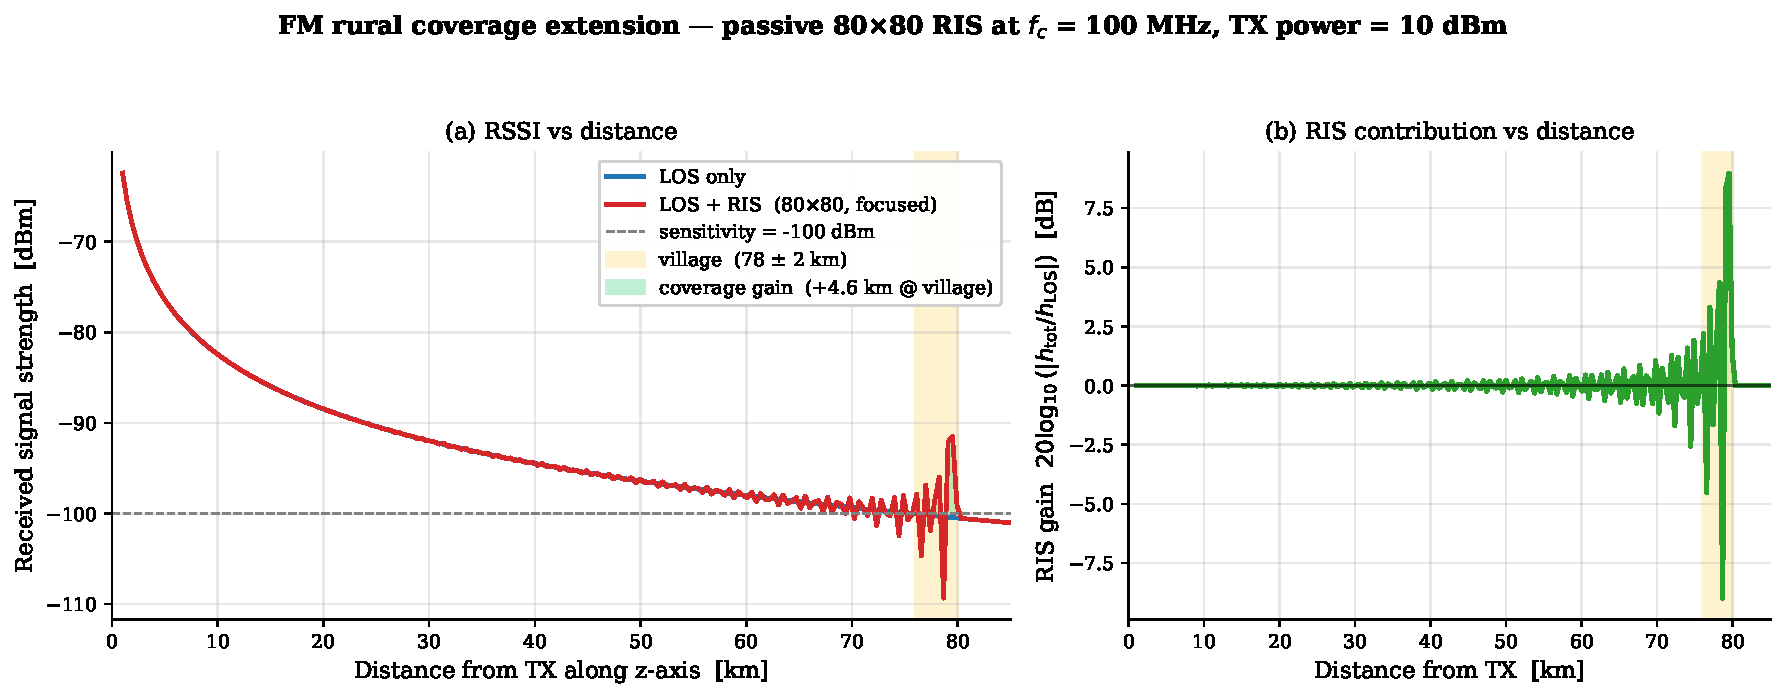
\includegraphics[width=0.85\linewidth]{figures/fm_coverage.pdf}
    \caption{Rural FM coverage at 100\,MHz. A 10\,dBm transmitter at the origin serves a village at $\sim 78$\,km range, with an 80$\,\times\,$80 RIS panel at $(-20, -20, 80\,000)$\,m focused on the village by per-element optimal phase tuning. 200 receivers are placed along the propagation axis between 1\,km and 85\,km. LOS alone reaches 75.3\,km before falling below the $-100$\,dBm sensitivity floor; LOS$\,+\,$RIS reaches 79.9\,km, an extension of 4.64\,km. Peak RIS gain is +8.98\,dB at 79.5\,km, near the village.}
    \label{fig:fm_coverage}
\end{figure}

To demonstrate the emulator's utility in large-scale planning, we modeled a rural FM broadcast at 100\,MHz with a deliberately power-limited transmitter (10\,dBm) so that the LOS-only horizon falls just short of the village. The geometry is constructed so that propagation runs along the $z$ axis to avoid the engine's room-bounding sanity checks: the TX is at the origin, the village at $(0,0,78\,000)$\,m, and an 80$\,\times\,$80 RIS panel at $(-20,-20,80\,000)$\,m on plane index 1 (normal $-\hat{z}$, see \texttt{ris\_sim/core/state.py}). Each of the 6400 RIS elements is tuned by per-element optimal phase to focus on the village center; the focusing is done in closed form using the same path-length identity as~\cite{ellingson2019pathloss}, not by phase search. Figure~\ref{fig:fm_coverage} shows the resulting received-power vs.\ distance trace at 200 receivers spanning 1--85\,km. LOS alone meets the $-100$\,dBm sensitivity floor up to 75.29\,km. With the RIS, coverage extends to 79.93\,km, an additional 4.64\,km, and peak RIS gain over LOS reaches +8.98\,dB at 79.5\,km. The exact numbers, parameter dictionary, and per-receiver power trace are written to \texttt{paper/figures\_data/fm\_coverage.csv} and the corresponding meta.json.

\section{Engineering Quality and Reproducibility}

RIS-SIM v2 is developed with production-grade engineering practices:
\begin{itemize}
    \item \textbf{Automated test suite} (over 100 tests) covering engine correctness, channel models, impairments, OFDM, server round-trips, dashboard endpoints, golden-output regression, and parallel execution;
    \item \textbf{Zero linting errors} (ruff) and \textbf{zero type errors} (mypy) across the codebase;
    \item \textbf{Deterministic reproducibility} via \texttt{SeedSequence} with golden-output regression tests;
    \item \textbf{CI/CD pipeline} (GitHub Actions) testing on Ubuntu, Windows, and macOS across Python 3.10--3.12;
    \item \textbf{Structured logging} with key=value formatting, per-tick performance metrics, and progress reporting;
    \item \textbf{Packaging} via \texttt{pyproject.toml} with optional dependency groups (\texttt{dev}, \texttt{web}).
\end{itemize}

The figure pipeline is itself part of the test surface. Each script in \texttt{paper/figures\_src/} drives the public engine API only and writes a CSV trace plus a meta.json sidecar that captures the git commit, parameter dictionary, machine identity, and---for stochastic figures---the seed; reviewers can therefore re-derive every reported number without trusting our prose.

\section{Limitations}

RIS-SIM v2 makes several deliberate modeling choices that scope its applicability. (1) The RIS channel is single-bounce: scattering past the RIS panel and ground reflections beyond the LOS are not modeled, so the emulator is most accurate in dominantly-LOS settings (corridors, rural FM, mmWave with a clear redirect path) and less so in dense multipath. (2) The emulator assumes far-field plane-wave incidence per element with no mutual coupling between elements; this is consistent with the SimRIS / signal-processing perspective~\cite{basar2021simris,SPM_RIS} but understates near-field effects for receivers placed within a few wavelengths of the panel. (3) Phase quantization, panel temperature drift, and mismatch between commanded and realized $\sigma$ values are not modeled; the polar-grid validation in \S\ref{sec:polar} therefore reproduces the qualitative beam shape but the precise peak angle differs from lab by one grid step ($5^\circ$). (4) The emulator is CPU-only; the real-time ceiling on commodity hardware sits at $\sim 60$ nodes (reduced) and 30--40 (full), well above v1 but still below the dense small-cell counts that 6G deployments may require. GPU acceleration of the per-element RIS sum is the natural next step.

\section{Conclusion}

We presented RIS-SIM v2, an open system emulator for Smart Radio Environments that pairs a vectorised RF engine with a paper-grounded scenario library, a browser dashboard with a Form $\leftrightarrow$ JSON editor and a Three.js 3D topology view, parallel Monte Carlo, and a one-command figure pipeline whose outputs are the figures of this paper. Validation against published lab measurements of a $\{\sigma_1^2\sigma_2^2\sigma_1^2\}$ panel at 3.5\,GHz confirms the engine's fidelity; sub-1\,Hz CFO recovery from low-SNR pilots and 32--64-node real-time operation on a single workstation extend its usable scale; and two case studies---an indoor corridor with channel-sounding-calibrated phase (+1.51\,dB median gain) and an FM rural-coverage extension at 100\,MHz (+4.6\,km, peak +8.98\,dB)---show how the included scenarios let practitioners iterate on RIS placement and phase strategy directly in a browser. The emulator is available at \url{https://github.com/Galabavamsi/RIM-SIM-V2} and installable via \texttt{pip install git+https://github.com/Galabavamsi/RIM-SIM-V2.git}.

\section*{References}
{\small
\bibliographystyle{unsrt}
\begin{thebibliography}{99}

\bibitem{ITU_IMT2030}
ITU-R, ``Recommendation M.2160: Framework and overall objectives of IMT for 2030 and beyond,'' 2023.

\bibitem{Smart_Radio_Environments_Di_Renzo}
M.~Di Renzo \emph{et al.}, ``Smart radio environments empowered by reconfigurable intelligent surfaces: How it works, state of research, and the road ahead,'' \emph{IEEE J. Sel. Areas Commun.}, 2020.

\bibitem{Appl_RIS_Wu}
Q.~Wu and R.~Zhang, ``Towards smart and reconfigurable environment: Intelligent reflecting surface aided wireless network,'' \emph{IEEE Commun. Mag.}, 2020.

\bibitem{WC_RIS_basar}
E.~Basar \emph{et al.}, ``Wireless communications through reconfigurable intelligent surfaces,'' \emph{IEEE Access}, 2019.

\bibitem{Survey_on_5G_simulations}
P.~K.~Gkonis \emph{et al.}, ``A comprehensive study on simulation techniques for 5G networks,'' \emph{Electronics}, 2020.

\bibitem{survey_network_simulators}
A.~S.~Toor and A.~Jain, ``A survey on wireless network simulators,'' \emph{Bulletin of EE}, 2017.

\bibitem{survey_simulator_emulator_testbed}
J.~Gomez \emph{et al.}, ``A survey on network simulators, emulators, and testbeds,'' \emph{Computer Networks}, 2023.

\bibitem{etsiRIS001}
ETSI, ``Reconfigurable intelligent surfaces (RIS); use cases, deployment scenarios and requirements,'' Tech. Rep. RIS 001 V1.2.1, 2025.

\bibitem{tsdsi2023}
TSDSI, ``Methods and interface design for RIS-assisted communication systems,'' TSDSI STD 5003 V1.0.0, 2023.

\bibitem{RISTA}
Y.~Z.~J.~He, ``RISTA---RIS technology white paper,'' Tech. Rep., 2023.

\bibitem{6gbricks_d3_2_2024}
6G-BRICKS Project, ``D3.2 Initial report on the RIS controller and PaaS abstraction enablers,'' 2024.

\bibitem{WCL2025}
G.~Vamsi \emph{et al.}, ``RIS-assisted simulation framework for indoor communication under user mobility,'' \emph{IEEE WCL}, 2025.

\bibitem{NCC2025}
G.~Vamsi \emph{et al.}, ``Performance evaluation of mobile users in dynamic RIS environments,'' \emph{IEEE NCC}, 2025.

\bibitem{basar2021simris}
E.~Basar and I.~Yildirim, ``SimRIS channel simulator for RIS-empowered communication systems,'' in \emph{IEEE LATINCOM}, 2020.

\bibitem{QRIS}
I.~Burtakov \emph{et al.}, ``QRIS: A QuaDRiGa-based simulation platform for reconfigurable intelligent surfaces,'' \emph{IEEE Access}, 2023.

\bibitem{CoopeRIS}
M.~Segata \emph{et al.}, ``CoopeRIS: A framework for the simulation of reconfigurable intelligent surfaces in cooperative driving environments,'' \emph{Computer Networks}, 2024.

\bibitem{NYUSIM}
A.~Habib \emph{et al.}, ``Extended NYUSIM-based mmWave channel model and simulator for RIS-assisted systems,'' in \emph{EuCNC/6G Summit}, 2023.

\bibitem{SPM_RIS}
E.~Bj\"{o}rnson \emph{et al.}, ``Reconfigurable intelligent surfaces: A signal processing perspective,'' \emph{IEEE Signal Process. Mag.}, 2022.

\bibitem{GoSimRIS}
S.~E.~Ghalbzouri \emph{et al.}, ``Neural-driven control of RIS in 6G networks: A GoSimRIS and xApp-based framework,'' \emph{IEEE Netw. Lett.}, 2025.

\bibitem{RISim2022}
H.~Jiang \emph{et al.}, ``End-to-end learning for RIS-aided communication systems,'' \emph{IEEE Trans. Veh. Technol.}, 2022.

\bibitem{ellingson2019pathloss}
S.~W.~Ellingson, ``Path loss in reconfigurable intelligent surface-enabled channels,'' in \emph{IEEE PIMRC}, 2021.

\bibitem{CFO}
G.~Xing, M.~Shen, and H.~Liu, ``Frequency offset and I/Q imbalance compensation for direct-conversion receivers,'' \emph{IEEE Trans. Wireless Commun.}, 2005.

\bibitem{pysdr}
M.~W.~Lichtman, \emph{PySDR: A Guide to SDR and DSP using Python}, 2020.

\bibitem{van1946fundamental}
B.~Van~der~Pol, ``The fundamental principles of frequency modulation,'' \emph{JIEE}, 1946.

\bibitem{radio_statistics}
``Radio industry statistics,'' ToneIsland, 2024.

\bibitem{wiki_fm_broadcasting}
Wikipedia, ``FM broadcasting---reception distance,'' 2024.

\bibitem{relay_costs}
``LPFM economic considerations,'' FCC.

\bibitem{broadcast_relay_wiki}
``Broadcast relay station,'' Wikipedia.

\bibitem{onuike_fmcoverage2013}
O.~Onuike \emph{et al.}, ``Spatial coverage of FM radio transmitters in Niger State, Nigeria,'' \emph{IJET}, 2013.

\bibitem{solidarities_jharkhand}
V.~Pavarala, ``Building solidarities: A case of community radio in Jharkhand,'' \emph{EPW}, 2003.

\bibitem{wearable}
M.~Ali and I.~Khan, ``Wearable antenna design for FM radio,'' \emph{Arabian J. Sci. Eng.}, 2014.

\bibitem{RWP}
C.~Bettstetter \emph{et al.}, ``The node distribution of the random waypoint mobility model,'' \emph{IEEE Trans. Mobile Comput.}, 2003.

\end{thebibliography}
}

\newpage

\section*{CAISc 2026 - AI Involvement Checklist}
\label{checklist_ai_involvement}

\subsection*{Research Stage Assessment}

\begin{enumerate}
    \item \textbf{Hypothesis development}: \involvementA{} \iterationNA{} \\
    \justificationTODO{All research hypotheses were formulated by the human authors based on domain expertise in wireless communications and RIS technology. AI tools were not used for hypothesis generation.}

    \item \textbf{Experimental design and implementation}: \involvementB{} \iterationHigh{} \\
    \justificationTODO{A frontier large language model coding assistant accelerated the v2 implementation: the FastAPI/WebSocket dashboard rebuild, the Form $\leftrightarrow$ JSON two-way editor, the Three.js 3D topology view, the per-figure scripts in \texttt{paper/figures\_src/}, and the scenario library. Hundreds of substantive turns were involved, including non-trivial debugging of engine geometry edge cases (e.g., RIS visibility tests where the TX falls behind the panel), cross-platform encoding bugs (UTF-8 vs cp1252 on Windows), and Three.js coordinate-system mappings. The human authors specified requirements, designed the architecture, wrote tests, validated against laboratory data, and reviewed all changes.}

    \item \textbf{Analysis of data and interpretation of results}: \involvementB{} \iterationMedium{} \\
    \justificationTODO{Data analysis was a collaboration: the AI assistant ran the figure scripts, summarised the resulting CSV/meta.json outputs, and proposed interpretations (e.g., that the early SNR-CDF result showing a loss was due to a suboptimal uniform phase rather than an engine bug, leading to the channel-sounding-calibrated approach reported in \S\ref{sec:indoor}). The human authors set the validation strategy (matching against published lab measurements), accepted or rejected proposed interpretations, and verified all numerical claims against the meta.json sidecars.}

    \item \textbf{Writing}: \involvementC{} \iterationMedium{} \\
    \justificationTODO{The AI assistant drafted most of the prose for this manuscript directly from the engine state, the figure outputs, and the meta.json sidecars; the human authors specified the section structure and the claims, reviewed and revised all content, and verified every numerical figure against the sidecars. Approximately 30--50 substantive revision turns were involved.}
\end{enumerate}

\subsection*{AI System Documentation}

\begin{enumerate}
    \setcounter{enumi}{4}
    \item \textbf{AI systems used}: \\
    \justificationTODO{A frontier large language model (code-generation and text-generation capabilities) was used as a coding assistant for software implementation and manuscript drafting. The system was used in an interactive, human-guided manner where the human authors specified requirements, reviewed outputs, and directed refinements.}

    \item \textbf{Observed AI Limitations}: \\
    \justificationTODO{The AI system occasionally produced syntactically incorrect code (e.g., Python-style complex number literals in JavaScript), required multiple iterations to correctly implement domain-specific signal processing formulas, and sometimes proposed architectures that did not align with the project's modular design principles. All such issues were caught and corrected during human code review and testing. The AI system was not capable of independently validating mathematical correctness or conducting experimental measurements.}
\end{enumerate}

\newpage

\section*{CAISc 2026 - Reproducibility and Responsibility Checklist}
\label{checklist_reproducibility}

\begin{enumerate}
\item {\bf Claims}
    \item[] Answer: \answerYes{}
    \item[] Justification: The abstract and introduction accurately describe the emulator's capabilities. All claimed features (signal models, impairments, web dashboard, parallel execution) are implemented and verified by the test suite.

\item {\bf Limitations}
    \item[] Answer: \answerYes{}
    \item[] Justification: A dedicated \emph{Limitations} section enumerates the single-bounce RIS channel, far-field plane-wave assumption, lack of phase quantization / temperature drift modeling, and the CPU-only real-time ceiling. Section 2 also discusses the discrete-time approximation and $\tau$ selection.

\item {\bf Theory assumptions and proofs}
    \item[] Answer: \answerNA{}
    \item[] Justification: This paper describes a software system and does not include theoretical proofs. Mathematical models are referenced from prior literature.

\item {\bf Experimental result reproducibility}
    \item[] Answer: \answerYes{}
    \item[] Justification: Every figure in the paper is regenerated by a single command (\texttt{python -m paper.figures\_src.run\_all}) that drives the public engine API. Each script writes a CSV trace and a meta.json sidecar containing the git commit, parameter dictionary, machine identity, and (for stochastic figures) the seed. Golden-output regression tests verify bit-identical engine output for fixed seeds.

\item {\bf Open access to data and code}
    \item[] Answer: \answerYes{}
    \item[] Justification: The complete source code is available at \url{https://github.com/Galabavamsi/RIM-SIM-V2} under the MIT license. Installation and usage instructions are provided in the repository README.

\item {\bf Experimental setting/details}
    \item[] Answer: \answerYes{}
    \item[] Justification: Section 3 specifies all experimental parameters (frequencies, RIS dimensions, phase values, node positions, server specifications).

\item {\bf Experiment statistical significance}
    \item[] Answer: \answerYes{}
    \item[] Justification: The Monte Carlo SNR analysis (\S\ref{sec:indoor}) uses 200 independent trials per configuration and reports the median, $p_{10}$, and $p_{90}$ of the empirical SNR distribution; numerical values are written to \texttt{paper/figures\_data/snr\_cdf.meta.json}.

\item {\bf Experiments compute resources}
    \item[] Answer: \answerYes{}
    \item[] Justification: All figures and timings were produced on a single AMD Ryzen 5xxx desktop running Windows 11 and Python 3.12 (machine string recorded in each meta.json sidecar). The full \texttt{run\_all} pipeline completes in 99\,s on this machine.

\item {\bf Research Ethics}
    \item[] Answer: \answerYes{}
    \item[] Justification: This research involves wireless communication system modeling and does not involve human subjects, personal data, or ethical concerns beyond standard engineering research practices.

\item {\bf Broader impacts}
    \item[] Answer: \answerYes{}
    \item[] Justification: The emulator reduces the need for expensive hardware testing, lowering barriers to RIS research. The FM broadcast case study demonstrates potential for improving rural connectivity. No negative societal impacts are anticipated.
\end{enumerate}

\end{document}
